% ============================================================================
% Fichier  : partie2/P02_C10_simulation.tex
% Titre    : Simuler : Monte-Carlo et Sensibilité
% Auteur   : MINKA MI NGUIDJOÏ Thierry Emmanuel
% Version  : 1.0 -- novembre 2026
% ============================================================================
% Sources : IEC 31010:2019 (simulation de Monte-Carlo) ; Hubbard et Seiersen
% (2016). Résultats : 100 000 années simulées (loi de Poisson pour le nombre
% d'événements, loi log-normale de médiane 290 et de 90e centile 540 millions
% pour chaque perte) ; valeurs calculées et vérifiées.
% ============================================================================

\chapter{Simuler : Monte-Carlo et Sensibilité}
\label{chap:simulation}
\chaptermark{Monte-Carlo et sensibilité}

\epigraph{%
    « La moyenne d'un fleuve est d'un mètre~;\\
    on s'y noie pourtant. »%
}{Proverbe repris par les statisticiens}

\niveauChapitre{Expert}{Chapitres~\ref{chap:risque}
et~\ref{chap:quantitatif}~; notions de lois de probabilité.}

\begin{boxobjectifs}
\begin{itemize}
    \item Expliquer le principe d'une simulation de Monte-Carlo appliquée
          aux pertes.
    \item Choisir des lois pour le nombre d'événements et pour l'ampleur
          d'une perte.
    \item Lire une distribution de pertes annuelles~: moyenne, centiles,
          probabilité de dépasser un seuil.
    \item Vérifier une appétence exprimée en probabilité.
    \item Identifier, par une analyse de sensibilité, les hypothèses qui
          comptent.
\end{itemize}
\end{boxobjectifs}

\bigskip

% ============================================================================
\section*{Question directrice : LiZbiZ respecte-t-elle son appétence « neuf ans sur dix »~?}
% ============================================================================

Le conseil a fixé~: « perte annuelle liée aux incidents informatiques
inférieure à 100~millions de FCFA dans neuf ans sur dix ». La perte
annuelle attendue de R-02, avec second facteur, est de 20~millions.
L'appétence est-elle respectée~? La moyenne ne le dit pas~: il faut la
distribution.

\medskip
\textbf{Plan du chapitre.}
\begin{enumerate}
    \item Le principe (section~\ref{sec:c10-principe}).
    \item Choisir les lois (section~\ref{sec:c10-lois}).
    \item Lire les résultats (section~\ref{sec:c10-resultats}).
    \item La courbe de dépassement (section~\ref{sec:c10-courbe}).
    \item L'analyse de sensibilité (section~\ref{sec:c10-sensibilite}).
\end{enumerate}

\separateur

% ============================================================================
\section{Le Principe}
\label{sec:c10-principe}
% ============================================================================

\begin{boxdef}
\termecle{Simulation de Monte-Carlo}~: méthode qui tire au hasard, un
grand nombre de fois, des valeurs des facteurs incertains selon leurs lois,
calcule pour chaque tirage le résultat, et étudie la distribution des
résultats obtenus.
\end{boxdef}

\begin{boxprocedure}
\textbf{Simuler une année de pertes, cent mille fois}
\begin{enumerate}
    \item Tirer le nombre d'événements de l'année selon une loi de
          fréquence.
    \item Pour chaque événement, tirer une perte selon une loi d'ampleur.
    \item Additionner les pertes de l'année.
    \item Recommencer cent mille fois.
    \item Trier les cent mille années et lire la moyenne, les centiles et
          la part des années au-dessus de chaque seuil.
\end{enumerate}
\end{boxprocedure}

% ============================================================================
\section{Choisir les Lois}
\label{sec:c10-lois}
% ============================================================================

\begin{tableaucours}{L{3.0cm}L{3.6cm}L{5.6cm}}{%
    \tableauHeader{Grandeur} &
    \tableauHeader{Loi usuelle} &
    \tableauHeader{Pourquoi}
}
Nombre d'événements par an & Poisson de paramètre $\lambda$ & Événements
indépendants, rares~; $\lambda$ = fréquence moyenne (LEF) \\
Perte par événement & Log-normale & Toujours positive, asymétrique~:
beaucoup de pertes modérées, quelques très grosses \\
Facteur estimé par trois points & PERT ou triangulaire & Bornée, centrée sur
la valeur la plus probable \\
\end{tableaucours}
\vspace{-0.8em}
\begin{center}{\small\itshape Tableau~10.1. Les lois d'une simulation de pertes}\end{center}

Pour R-02, LiZbiZ retient une loi de Poisson de paramètre $0{,}29$ (sans
second facteur) ou $0{,}062$ (avec), et une perte log-normale de médiane
290~millions et de 90\textsuperscript{e}~centile 540~millions, dont la
moyenne (326~millions) est celle de l'estimation FAIR.

% ============================================================================
\section{Lire les Résultats}
\label{sec:c10-resultats}
% ============================================================================

\begin{tableaucours}{L{6.2cm}R{2.8cm}R{2.8cm}}{%
    \tableauHeader{Sur 100\,000 années simulées} &
    \tableauHeader{Sans second facteur} &
    \tableauHeader{Avec second facteur}
}
Perte annuelle moyenne & 94 & 20 \\
Part des années avec au moins une perte & 25,0~\% & 6,0~\% \\
90\textsuperscript{e} centile & 367 & 0 \\
95\textsuperscript{e} centile & 517 & 184 \\
99\textsuperscript{e} centile & 863 & 482 \\
Part des années au-delà de 100~millions & 24,7~\% & 5,9~\% \\
Part des années au-delà de 500~millions & 5,4~\% & 0,9~\% \\
\end{tableaucours}
\vspace{-0.8em}
\begin{center}{\small\itshape Tableau~10.2. Distribution des pertes annuelles de R-02 (millions de FCFA)}\end{center}

\begin{boxscenario}{Opération LIZBIZ. L'appétence vérifiée}
\textbf{Constatation.} Sans second facteur, une année sur quatre environ
(24,7~\%) dépasse 100~millions~; avec second facteur, environ une sur
dix-sept (5,9~\%).

\medskip
\textbf{Analyse} (confiance moyenne). L'appétence « moins de 100~millions
neuf ans sur dix » demande moins de 10~\% d'années au-delà du seuil. Elle
n'était pas respectée sans second facteur~; elle l'est avec, pour ce seul
risque. Il faut encore ajouter les autres risques numériques du registre
pour conclure sur l'ensemble.
\end{boxscenario}

\begin{boxalert}
\textbf{Violation typique.} Lire le 90\textsuperscript{e} centile « 0 »
comme « aucun risque ».

\smallskip
\textbf{Règle~:} avec second facteur, plus de 90~\% des années sont sans
perte, d'où un 90\textsuperscript{e} centile nul~; mais le
95\textsuperscript{e} centile atteint 184~millions. Un risque rare se lit
dans les centiles élevés et dans la probabilité de dépassement.
\end{boxalert}

% ============================================================================
\section{La Courbe de Dépassement}
\label{sec:c10-courbe}
% ============================================================================

\begin{boxdef}
\termecle{Courbe de dépassement des pertes}~: courbe qui donne, pour chaque
montant, la probabilité que la perte annuelle le dépasse. On la compare à
la \emph{courbe de tolérance} du conseil.
\end{boxdef}

\begin{center}
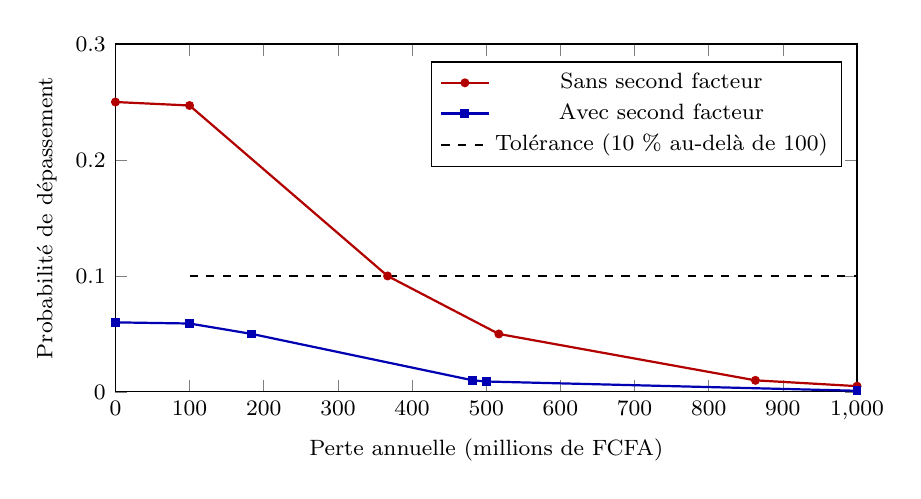
\begin{tikzpicture}
\begin{axis}[width=11cm, height=6cm, xmin=0, xmax=1000, ymin=0, ymax=0.3,
    xlabel={Perte annuelle (millions de FCFA)}, ylabel={Probabilité de dépassement},
    yticklabel style={/pgf/number format/fixed, /pgf/number format/precision=2},
    legend style={font=\footnotesize, at={(0.98,0.95)}, anchor=north east},
    tick label style={font=\footnotesize}, label style={font=\footnotesize}]
\addplot[thick, red!70!black, mark=*, mark size=1.2pt] coordinates
    {(0,0.25) (100,0.247) (367,0.10) (517,0.05) (863,0.01) (1000,0.005)};
\addplot[thick, blue!70!black, mark=square*, mark size=1.2pt] coordinates
    {(0,0.06) (100,0.059) (184,0.05) (482,0.01) (500,0.009) (1000,0.001)};
\addplot[thick, dashed, black] coordinates {(100,0.10) (1000,0.10)};
\legend{Sans second facteur, Avec second facteur, Tolérance (10~\% au-delà de 100)}
\end{axis}
\end{tikzpicture}
\end{center}
\vspace{-0.4em}
\begin{center}{\small\itshape Figure~10.1. Courbes de dépassement de R-02 (points issus du Tableau~10.2)}\end{center}

% ============================================================================
\section{L'Analyse de Sensibilité}
\label{sec:c10-sensibilite}
% ============================================================================

Quelles hypothèses comptent le plus~? On fait varier chacune entre ses
bornes plausibles, les autres restant fixes, et l'on observe la perte
annuelle moyenne.

\begin{tableaucours}{L{5.4cm}L{3.2cm}R{3.4cm}}{%
    \tableauHeader{Hypothèse (sans second facteur)} &
    \tableauHeader{Plage} &
    \tableauHeader{Perte moyenne}
}
Fréquence $\lambda$ & 0,20 à 0,40 & 65 à 130 \\
Médiane de la perte & 200 à 380 & 65 à 124 \\
\end{tableaucours}
\vspace{-0.8em}
\begin{center}{\small\itshape Tableau~10.3. Sensibilité de la perte moyenne (millions de FCFA)}\end{center}

\textbf{Analyse.} Les deux hypothèses pèsent autant. Mais la décision (le
second facteur) agit sur la fréquence, qu'elle divise par près de cinq~:
c'est elle qu'il faut vérifier en priorité, par l'indicateur de
couverture du second facteur. Une analyse de sensibilité dit où dépenser
l'effort de mesure.

\begin{boxmetier}{Gestionnaire de risques}
\textbf{Publier le code et les hypothèses.} Mme~MOUAFO conserve le
programme de simulation, les lois, les paramètres et la graine du tirage
aléatoire~: un tiers doit pouvoir refaire le calcul et obtenir les mêmes
chiffres.
\end{boxmetier}

\begin{boxmetier}{Auditeur des systèmes d'information}
\textbf{Refaire un point.} L'auditeur ne refait pas toute la simulation~;
il vérifie un résultat simple, par exemple que la moyenne est proche de
$\lambda \times$ perte moyenne ($0{,}29 \times 326 \approx 94$).
\end{boxmetier}

\separateur

\begin{boxresume}
\textbf{Ce qu'il faut retenir de ce chapitre~:}
\begin{itemize}
    \item \textbf{Monte-Carlo} tire des milliers d'années et en étudie la
          distribution.
    \item \textbf{Poisson} pour le nombre d'événements, \textbf{log-normale}
          pour l'ampleur.
    \item \textbf{Les centiles et la probabilité de dépassement} disent la
          pire année, que la moyenne cache.
    \item \textbf{La courbe de dépassement} se compare à la tolérance du
          conseil.
    \item \textbf{La sensibilité} dit quelles hypothèses vérifier d'abord.
\end{itemize}
\end{boxresume}

\begin{boxinfo}
\textbf{Points de contrôle de l'élève.} Je sais~: décrire les étapes d'une
simulation~; choisir les lois~; lire moyenne, centiles et probabilités de
dépassement~; vérifier une appétence en probabilité~; mener une analyse de
sensibilité.
\end{boxinfo}

\bigskip

\begin{boxexo}[title={\ding{45}\quad Exercice~10.1. Les étapes \niveaubase}]
Décrivez, en cinq lignes, ce que fait la simulation pour une seule année.
\end{boxexo}

\begin{boxexo}[title={\ding{45}\quad Exercice~10.2. Lire \niveaubase}]
D'après le Tableau~10.2, sans second facteur, combien d'années sur cent
dépassent 500~millions~?
\end{boxexo}

\begin{boxexo}[title={\ding{45}\quad Exercice~10.3. Poisson \niveaubase}]
Avec $\lambda = 0{,}29$, quelle est la probabilité d'une année sans aucun
événement~? Comparez au tableau.
\end{boxexo}

\begin{boxexo}[title={\ding{45}\quad Exercice~10.4. Le centile nul \niveaumoyen}]
Expliquez pourquoi le 90\textsuperscript{e} centile est nul avec second
facteur, alors que le 95\textsuperscript{e} atteint 184~millions.
\end{boxexo}

\begin{boxexo}[title={\ding{45}\quad Exercice~10.5. L'appétence \niveaumoyen}]
Montrez, à partir du Tableau~10.2, que l'appétence est respectée avec
second facteur et ne l'est pas sans.
\end{boxexo}

\begin{boxexo}[title={\ding{45}\quad Exercice~10.6. Vérifier la moyenne \niveaumoyen}]
Vérifiez que les moyennes du Tableau~10.2 sont cohérentes avec les
estimations FAIR du Chapitre~\ref{chap:quantitatif}.
\end{boxexo}

\begin{boxexo}[title={\ding{45}\quad Exercice~10.7. Pourquoi log-normale \niveaumoyen}]
Pourquoi une loi normale conviendrait-elle mal à l'ampleur d'une perte~?
\end{boxexo}

\begin{boxexo}[title={\ding{45}\quad Exercice~10.8. Sensibilité \niveaumoyen}]
Si la fréquence réelle sans second facteur était de 0,40, l'appétence
serait-elle encore plus loin d'être respectée~? Justifiez.
\end{boxexo}

\begin{boxexo}[title={\ding{45}\quad Exercice~10.9. Plusieurs risques \niveauexpert}]
Décrivez comment simuler ensemble les cinq risques numériques majeurs de
LiZbiZ pour vérifier l'appétence globale. Quelle difficulté pose leur
éventuelle dépendance~?
\end{boxexo}

\begin{boxexo}[title={\ding{45}\quad Exercice~10.10. Programmer \niveauexpert}]
Écrivez, en Python ou dans un tableur, une simulation de 10\,000 années
pour R-02 avec second facteur, et comparez vos résultats au
Tableau~10.2.
\end{boxexo}

\bigskip

\begin{boxinfo}
\textbf{Pour aller plus loin.}
\begin{itemize}
    \item IEC~31010, fiche sur la simulation de Monte-Carlo~\cite{iec31010}.
    \item D.~Hubbard et R.~Seiersen~\cite{hubbard2016cyber}.
\end{itemize}
\end{boxinfo}

\begin{boxinfo}
\textbf{Transition.} Estimer ne suffit pas~: il faut traiter, suivre et
rendre compte. C'est l'objet du Chapitre~\ref{chap:traiter}.
\end{boxinfo}
